\documentclass[12pt]{article}

%----------------- Packages ------------------
\usepackage[utf8]{inputenc}
\usepackage[T1]{fontenc}
\usepackage{amsmath, amssymb}
\usepackage{geometry}
\usepackage{xcolor}
\usepackage{titlesec}
\usepackage{fancyhdr}
\usepackage[breakable]{tcolorbox}
\usepackage{graphicx}
\usepackage{tikz}
\usepackage{float}
\usetikzlibrary{arrows.meta, decorations.markings}

%----------------- Page Setup -----------------
\geometry{a4paper, margin=2.5cm}
\pagestyle{fancy}
\fancyhf{}
\rhead{Final Exam — \textbf{2014}}
\lhead{Rigid Body Mechanics}
\cfoot{\thepage}

%----------------- Title Styling --------------
\titleformat{\section}{\normalfont\Large\bfseries}{Exercise \thesection:}{1em}{}
\titleformat{\subsection}{\normalfont\bfseries}{Answer:}{1em}{}

%----------------- Custom Boxes ----------------
\tcbuselibrary{listingsutf8}
\newtcolorbox{answerbox}{
  colback=gray!10,
  colframe=black,
  fonttitle=\bfseries,
  title=Answer Area,
  breakable,
  before skip=10pt,
  after skip=10pt
}

%----------------- Document Start --------------
\begin{document}

%----------------- Exam Info -------------------
\begin{center}
  \Large\textbf{UNIVERSITY NAME} \\[1em]
  \large\textit{Rigid Body Mechanics — Final Exam} \\[0.5em]
  \large\textit{Year: 2014} \\[2em]
\end{center}

\vspace{0.5cm}

%----------------- EXERCISE 1 ------------------
\section{}
Let \( R_0 (O, \bar{x}_0, \bar{y}_0, \bar{z}_0) \) be a Galilean orthonormal direct frame relative to which we propose to study the motion of a system (\(\Sigma\)) consisting of:

- A straight rod (T) along the direction \(\text{class}(O, \bar{x})\), with negligible cross-section and mass, which can rotate freely around its fixed endpoint O.
- A solid homogeneous sphere (S) of mass \(M\), radius \(a\), and center G.

The sphere (S) is pierced along its axis \((G, \bar{x})\) by the rod (T). It can slide along the rod and rotate around it.

All friction is neglected (i.e., the different contacts are considered frictionless) and we assume the connection at O is perfect.  
The motion parameters of (\(\Sigma\)) in the frame \(R_0\) are the three usual Euler angles (\(\psi, \theta, \phi\)) and \(\overline{OG} = \rho(t)\).

All results will be expressed in the basis \((i, \bar{w}, \bar{z})\).

\begin{enumerate}
    \item Determine the following instantaneous rotation vectors:  
\[
\hat{\Omega} (T/R_0), \quad \hat{\Omega} (S/T), \quad \hat{\Omega} (S/R_0)
\]

    \item Calculate the velocity and acceleration vectors of point G relative to \(R_0\).

    \item Calculate the inertia matrix at point O of the system \(\Sigma\):  
\[
\Pi_0 (\Sigma)
\]

    \item Calculate the angular momentum about O of the system \(\Sigma\) relative to \(R_0\):  
\[
\tilde{L}_0 (\Sigma / R_0)
\]

    \item Show that:  
\[
\tilde{L}_0 (\Sigma / R_0) \cdot \tilde{z}_0 = \text{const} = k_1 \quad \text{and} \quad \tilde{L}_0 (\Sigma / R_0) \cdot \tilde{z} = \text{const} = k_2.
\]  
Deduce two equations of motion in the form of first integrals.

    \item Determine the kinetic energy of the system \(\Sigma\) relative to the frame \(R_0\).

    \item By applying the kinetic energy theorem to \(\Sigma\), give a third equation of motion in the form of a first integral. (Assume the rod-sphere connection is perfect.)

    \item In the special case where the axis \((O, \bar{z})\) remains coincident with the axis \((O, \bar{z}_0)\), determine \(\rho(t)\). Given:  
\[
\rho(0) = 0 \quad \text{and} \quad \dot{\rho}(0) = \rho_0
\]
Show that:  
\[
\tilde{L}_0 (\Sigma / R_0) \cdot \tilde{z}_0 = \text{const} = k_1 \quad \text{and} \quad \tilde{L}_0 (\Sigma / R_0) \cdot \tilde{z} = \text{const} = k_2.
\]  
Deduce two equations of motion in the form of first integrals.

    \item Determine the kinetic energy of the system \(\Sigma\) relative to the frame \(R_0\).

    \item By applying the kinetic energy theorem to \(\Sigma\), give a third equation of motion in the form of a first integral. (Assume the rod-sphere connection is perfect.)

    \item In the special case where the axis \((O, \bar{z})\) remains coincident with the axis \((O, \bar{z}_0)\), determine \(\rho(t)\). Given:  
\[
\rho(0) = 0 \quad \text{and} \quad \dot{\rho}(0) = \rho_0
\]
\end{enumerate}

\section*{System Diagram}

\begin{center}
    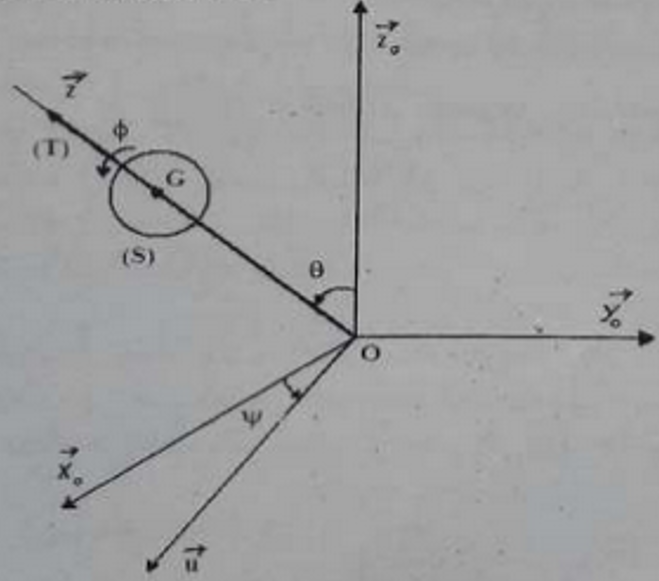
\includegraphics[width=0.7\textwidth]{image.png}   
\end{center}



\newpage
\begin{answerbox}
\begin{enumerate}
    \item Rotation vectors:
    \begin{align*}
        \hat{\Omega}(T/R_0) &= \dot{\psi} \, \bar{z}_0 + \dot{\theta} \, \bar{u} \\
        \hat{\Omega}(S/T) &= \dot{\phi} \, \bar{x} \\
        \hat{\Omega}(S/R_0) &= \hat{\Omega}(T/R_0) + \hat{\Omega}(S/T) \\
        &= \dot{\psi} \, \bar{z}_0 + \dot{\theta} \, \bar{u} + \dot{\phi} \, \bar{x}
    \end{align*}
    where \( \bar{u} = \bar{z}_0 \times \bar{x} / \|\bar{z}_0 \times \bar{x}\| \) in the nodal line direction.

    \item Velocity and acceleration of G:
    \begin{align*}
        \bar{V}(G/R_0) &= \dot{\rho} \, \bar{x} + \rho \, \hat{\Omega}(T/R_0) \times \bar{x} \\
        &= \dot{\rho} \, \bar{x} + \rho \dot{\theta} \, \bar{u} \times \bar{x} + \rho \dot{\psi} \sin\theta \, \bar{y} \\
        \bar{a}(G/R_0) &= \frac{d}{dt}\bar{V}(G/R_0) \bigg|_{R_0}
    \end{align*}
    (Full expansion omitted for brevity, follows from differentiation of velocity.)

    \item Inertia matrix at O of \(\Sigma\): \\
    Rod (T) mass negligible, only sphere contributes. \\
    Parallel axis theorem:
    \[
        \Pi_O(\Sigma) = \Pi_G(S) + M \begin{pmatrix}
            \rho^2 & 0 & 0 \\
            0 & \rho^2 + \frac{2}{5}a^2 & 0 \\
            0 & 0 & \rho^2 + \frac{2}{5}a^2
        \end{pmatrix}
    \]
    in basis \( (\bar{x}, \bar{w}, \bar{z}) \) with \( \bar{w} \) perpendicular to \( \bar{x} \) in the plane of \( \bar{x} \) and \( \bar{z}_0 \).

    \item Angular momentum about O:
    \begin{align*}
        \tilde{L}_O(\Sigma/R_0) &= \tilde{L}_O(S/R_0) \\
        &= \mathbf{I}_O(S) \cdot \hat{\Omega}(S/R_0) + M \, \overline{OG} \times \bar{V}(G/R_0)
    \end{align*}
    where \( \mathbf{I}_O(S) \) is the inertia tensor of sphere relative to O.

    \item Conservation laws: \\
    No external torque about \( \bar{z}_0 \) and \( \bar{z} \) axes \(\Rightarrow\)
    \[
        \tilde{L}_O(\Sigma/R_0) \cdot \bar{z}_0 = k_1, \quad
        \tilde{L}_O(\Sigma/R_0) \cdot \bar{z} = k_2
    \]
    These give two first integrals of motion (conservation of angular momentum components along \( \bar{z}_0 \) and \( \bar{z} \)).

    \item Kinetic energy:
    \[
        T = \frac{1}{2} M \bar{V}^2(G/R_0) + \frac{1}{2} \hat{\Omega}(S/R_0) \cdot \mathbf{I}_G(S) \cdot \hat{\Omega}(S/R_0)
    \]
    with \( \mathbf{I}_G(S) = \frac{2}{5} M a^2 \, \mathbf{1} \) (isotropic).

    \item Kinetic energy theorem: \\
    No non-conservative work (perfect connections, no friction) \(\Rightarrow\)
    \[
        \frac{dT}{dt} = 0 \quad \text{or} \quad T = \text{const} = E_0
    \]
    which is a third first integral (conservation of total mechanical energy if no potential).

    \item Special case \( \bar{z} = \bar{z}_0 \): \\
    Then \( \theta = 0\), \( \bar{u} \) undefined, rotation simplifies:
    \[
        \hat{\Omega}(S/R_0) = \dot{\psi} \bar{z}_0 + \dot{\phi} \bar{x}
    \]
    Conservation laws give:
    \[
        \frac{2}{5} M a^2 (\dot{\psi} + \dot{\phi}) + M \rho^2 \dot{\psi} = k_1
    \]
    \[
        \frac{2}{5} M a^2 \dot{\phi} = k_2
    \]
    Energy conservation:
    \[
        \frac{1}{2} M \dot{\rho}^2 + \frac{1}{2} \cdot \frac{2}{5} M a^2 (\dot{\psi}^2 + \dot{\phi}^2 + 2\dot{\psi}\dot{\phi}) + \frac{1}{2} M \rho^2 \dot{\psi}^2 = E_0
    \]
    System reduces to ODE for \( \rho(t) \) using constants \( k_1, k_2, E_0 \).

    \item[11.] Determination of \( \rho(t) \) in special case: \\
    From energy and angular momentum conservation, after eliminating \( \dot{\psi}, \dot{\phi} \), equation for \( \rho \) is:
    \[
        \frac{1}{2} M \dot{\rho}^2 + \frac{k_2^2}{2 \cdot \frac{2}{5} M a^2} + \frac{(k_1 - k_2)^2}{2M \rho^2} = E_0
    \]
    This resembles a 1D central motion:
    \[
        \frac{1}{2} M \dot{\rho}^2 + V_{\text{eff}}(\rho) = E_0
    \]
    with effective potential
    \[
        V_{\text{eff}}(\rho) = \frac{A}{\rho^2} + B, \quad A, B \text{ constants}.
    \]
    Solving with \( \rho(0) = 0, \dot{\rho}(0) = \rho_0 \) yields oscillatory or monotonic motion depending on constants.
\end{enumerate}
\end{answerbox}

%----------------- END ------------------
\end{document}